In this paper we only consider the Wasserstein-1 distance, also called Earth-mover, and noted $\W$ for $\W_1$.
The $1$-Wasserstein distance between two probability distributions $\mu$ and $\nu$ in $\Omega$, and its dual formulation by Kantorovich-Rubinstein duality \cite{villani2008}, is defined as the solution of:
\begin{subequations}

\begin{align}
\W(\mu,\nu) & = \inf_{\pi \in \Pi(\mu,\nu)}\underset{x,z \sim \pi}{\mathbb{E}}\parallel \textbf{x}-\textbf{z} \parallel \label{wasserstein}\\
  & =\sup_{f \in Lip_1(\Omega)} \underset{\textbf{x} \sim \mu}{\mathbb{E}} \left[f(\textbf{x} )\right] -\underset{\textbf{x}  \sim \nu}{\mathbb{E}} \left[f(\textbf{x} )\right] \label{kantorovich}
\end{align}
\end{subequations}

where $\Pi(\mu,\nu)$ is the set of all probability measures on $\Omega\times \Omega$ with marginals $\mu$ and $\nu$ and $Lip_1(\Omega)$ denotes the space of 1-Lipschitz functions over $\Omega$. 
Although, the infimum in Eq.~\eqref{wasserstein} is not tractable in general, the dual problem can be estimated through the optimization of a regularized neural network. This approach has been introduced in WGAN  \cite{Arjovsky2017} where $Lip_1(\Omega)$ is approximated by the set of neural networks with bounded weights (better approximations of $Lip_1(\Omega)$ will be discussed in Section~\ref{sec:lip_const}). 

We consider a binary classification problem on feature vector space $X\subset \Omega$ and and labels $Y= \{-1,1\}$. We name $P_+=\mathbb{P}(X|Y=1)$ and  $P_-=\mathbb{P}(X|Y=-1)$, the conditional distributions with respect to Y. We note $p=P(Y=1)$ and $1-p=P(Y=-1)$ the apriori class distribution. The classification problem is balanced when $p=\frac{1}{2}$.\\

In WGAN, \cite{Arjovsky2017} proposed to use the learned neural network (denoted $\hat{f}$ in the following),  by maximizing the Eq.~\eqref{kantorovich}, as a discriminator between fake and real images, in analogy with GAN~\cite{Goodfellow2014}.
%\footnote{{\color{red} (FRANCK:proposition de reformulation, l'ancienne version est commentee)}} 
%In analogy with GAN~\cite{Goodfellow2014}, the function obtained by optimizing equation~\ref{kantorovich} (denoted $\hat{f}$ in the following) in WGAN behaves like a discriminator between fake and real examples. 
To build a classifier based on $\hat{f}$, one can simply note that if  $f^*$ is an optimal solution of Eq.~\eqref{kantorovich}, then  $f^* + C, C\in \mathbb{R}$, is also optimal. Centering the function $f^*$ (resp. $\hat{f}$), Eq.~\eqref{eq:wass_vanilla_classif}, enables classification according to the sign of $f_c^*(x)$ (resp.$\hat{f_c}$ for the empirical solution).
%\footnote{{\color{red} (FRANCK:idem, l'ancienne version est commentee)}} 
%Let $f^*$ is an optimal solution of Equation~\eqref{kantorovich}, then $f^* + c, c\in \mathbb{R}$, is also optimal. In order to build a classifier, the simplest solution consists in centering the function $f^*$ (resp. $\hat{f}$)  as follows:The class correspond to the sign of $f_c^*(x)$ (resp.$\hat{f_c}$ for the empirical solution). 
\begin{equation}
\label{eq:wass_vanilla_classif}
f_c^*(\textbf{x} )=f^*(\textbf{x} )-\frac{1}{2}\left(\underset{\textbf{z}  \sim P_+}{\mathbb{E}} \left[f^*(\textbf{z} )\right] +\underset{\textbf{z}  \sim P_-}{\mathbb{E}} \left[f^*(\textbf{z} )\right]\right).
\end{equation}

Such a classifier would exhibit good properties in terms of robustness for two main reasons: First, it has been shown in \cite{villani2008} that the function $f^*$ is directly related to the cost of transportation between two points linked by the transportation plan %(when $\pi^*(x=y)=0$) 
as follows:

%Let denote $\hat{f}$ the function obtained by optimizing equation~\ref{kantorovich} 
%In the balanced discrete case, it has been shown {\color{red} (FRANCK: Ref ?)} that the optimal transport plan is an 1-1 transportation plan (i.e. $\Pi^*_{i,j} \in\{0,1\}$) and:
%\begin{equation}
%\forall i,j\text{ s.a. }\Pi^*_{i,j}=1,  F^*_i-F^*_{n+j}= C_{i,j}
%\end{equation}
%where $F^*$ is the optimal solution of the dual optimal transport problem. 

\begin{equation}
\label{eq:transport_cost}
\mathbb{P}_{\textbf{x},\textbf{z}\sim \pi^*}(f^*(\textbf{x})-f^*(\textbf{z})=||\textbf{x}-\textbf{z}||)=1.
\end{equation}
 %This shows that the function $f^*$ is directly related to the cost of transportation between two point linked by the transportation plan. 
 Second, it was shown in \cite{gulrajani2017improved,pmlr-v97-anil19a}, that this optimal solution also induces a property stronger  than 1-Lipschitz:
\begin{equation}
\label{eq:nabla_1}
||\nabla f^* ||=1 \text{ almost surely on the support of }\pi^*.
\end{equation}
%The previous properties with respect to the transportation plan and the 1-Lipschitz constraint also underlined good properties in terms of robustness. 

However, applying this vanilla classifier (Eq.~\eqref{eq:wass_vanilla_classif}) to a toy dataset such as the two-moons problem, leads to a poor accuracy.
Indeed, Figures~\ref{wass:sub1} and~\ref{wass:sub2} present respectively the distribution of the values of $\hat{f_c}(x)$ conditionally to the classes and the level map of $\hat{f_c}$. We can observe that, even if the classes are easily separable, the distributions of the values of $\hat{f_c}$ conditionally to the class overlap. Thus, the 0-level threshold on $\hat{f_c}$ does not correspond to the optimal separator (even if it is better than random). Intuitively, $\hat{f_c}$  
%{\color{red} (FRANCK: $f*$?)} 
maximizes the difference of the expectancy of the image of  
the two distributions but do not try to minimize their overlap (Fig.~\ref{wass:sub1}). 
%We can also note %remark 
%that, for $\W$ 
%and the Earth-mover distance, 
%the solution is not unique.
%{\color{red} ( Thibaut ) on fait une analogie avec les WGAN avant de d'expliciter comment on fait la classification a partir de  f ( eq 11 ), ce qui risque plus d'embrouiller le lecteur. ( Entre le discriminateur d'un GAN, la régularization de Wasserstein d'un GAN et notre classifier, la confusion peut vite arriver )\\
%MAthieu -> exact!}\\
%{FRANCK -> yes tentative d'explicitation differente dans l'intro! plus qqes reofrmulations ci dessous}
%In analogy with GAN \cite{Goodfellow2014}, the network that computes the function $f$ with respect to Kantorovich-Rubinstein formulation in WGAN can be viewed as a classifier.  
%{\color{red}(MATHIEU) : faire l'exemple avec le transport optimal et le seuil)}

\begin{figure*}
\centering
\begin{subfigure}{.4\textwidth}
  \centering
  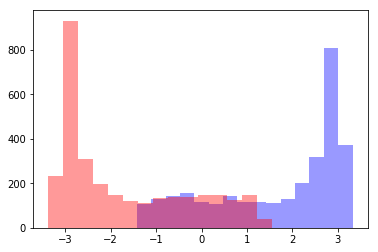
\includegraphics[width=1\linewidth]{img/wass_2moons_dist.png}
  \caption{Distribution of $\hat{f_c}$ conditionally to the classes}
  \label{wass:sub1}
\end{subfigure}%
\begin{subfigure}{.36\textwidth}
  \centering
  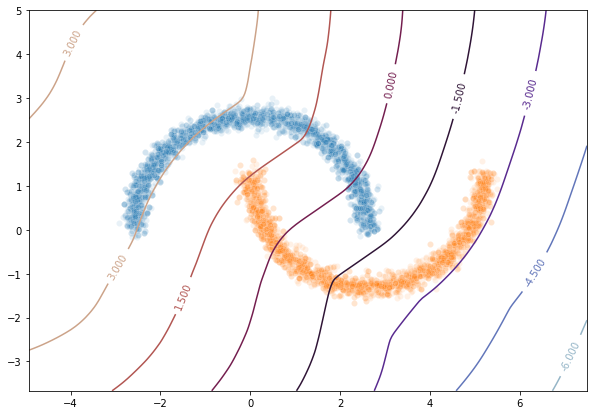
\includegraphics[width=1\linewidth]{img/wass_2moons_class.png}
  \caption{Level map of $\hat{f_c}$}
  \label{wass:sub2}
\end{subfigure}
\caption{Wasserstein classification (Eq.~\eqref{eq:wass_vanilla_classif}) on the two moons.}
\label{fig:wass}
\end{figure*}
